% =====================================================================================
%  ABC-Q v2 manuscript.
%  Written with the standard article class so it compiles anywhere. To submit to a
%  Springer Nature journal, download the Springer Nature LaTeX template (sn-jnl.cls),
%  replace the preamble below with  \documentclass[sn-mathphys-num]{sn-jnl}  and move the
%  title/author/abstract block into the template's \title/\author/\abstract macros.
% =====================================================================================
\documentclass[11pt,a4paper]{article}
\usepackage[margin=2.5cm]{geometry}
\usepackage[utf8]{inputenc}
\usepackage[T1]{fontenc}
\usepackage{lmodern}
\usepackage{amsmath,amssymb,amsthm}
\usepackage{booktabs,multirow,array}
\usepackage{graphicx}
\usepackage{algorithm}
\usepackage{algpseudocode}
\usepackage{xcolor}
\usepackage[numbers,sort&compress]{natbib}
\usepackage[hidelinks]{hyperref}
\usepackage{placeins}
\emergencystretch=3em

\newtheorem{proposition}{Proposition}
\newtheorem{remark}{Remark}
\newcommand{\B}{\mathcal{B}}

\title{Surrogate-Assisted Discrete Artificial Bee Colony Search for\\
Budget-Constrained Mixed-Precision Post-Training Quantization}

\author{Manav$^{1}$ \and Sarthak Jain$^{1}$ \and Manik Dhiman$^{1}$ \and Shreshth Varshney$^{1}$\\[4pt]
\small $^{1}$Netaji Subhas University of Technology, Delhi, India\\
\small Corresponding author: Manav (ORCID 0009-0005-5197-5195)}
\date{}

\begin{document}
\maketitle

\begin{abstract}
Mixed-precision post-training quantization assigns a bit-width to every layer of a trained network,
but choosing the assignment is a hard discrete optimisation problem. Swarm and evolutionary methods
are popular for it, yet are usually compared with penalised fitness functions that make methods land
at different costs. We pose bit allocation as accuracy maximisation under a hard bit-operations (BOPs)
budget with an equal evaluation budget for all methods, and propose ABC-Q v2, a surrogate-assisted
discrete Artificial Bee Colony search. It measures single-layer quantization damage directly, fits an
additive accuracy surrogate refined online by ridge regression towards these probes, seeds and
re-seeds food sources with exact multiple-choice-knapsack optima of randomly perturbed surrogates,
and explores with budget-neutral information-sharing moves. On ResNet-20 and MobileNetV2 trained on
CIFAR-10/100, two budgets and ten seeds, random search, a genetic algorithm, CMA-ES and our earlier
ABC-Q are, in 15 of 16 cases, \emph{worse} than uniform 4-bit quantization at the same cost, while
ABC-Q v2 attains the highest calibration accuracy in all eight settings (Holm-corrected Wilcoxon
$p=0.008$ against every search baseline) and improves test accuracy over uniform W4A4 by up to
$23.1$ percentage points (MobileNetV2/CIFAR-10). It also outperforms a HAWQ-V2-style one-shot
allocator, and we show that gradient- and Fisher-based sensitivity proxies are only moderately
correlated with measured damage. An ablation shows that probing, knapsack seeding and the online
surrogate carry the gains, whereas the colony dynamics add little at our budget, and short
quantization-aware fine-tuning reduces the differences between allocations to about one percentage
point. Code and all per-run results are released.
\end{abstract}

\noindent\textbf{Keywords:} mixed-precision quantization; artificial bee colony; surrogate-assisted
optimisation; multiple-choice knapsack; post-training quantization; edge inference

%% ===================================================================================
\section{Introduction}
%% ===================================================================================

Deploying convolutional networks on phones, microcontrollers and drones is constrained by memory,
energy and latency. Quantization maps 32-bit floating-point weights and activations to low-precision
integers and is the most widely deployed compression technique
\citep{Jacob2018,Krishnamoorthi2018,Nagel2021White,Gholami2021Survey}. Post-training quantization
(PTQ) is particularly attractive because it needs only a small unlabelled or labelled
\emph{calibration} set and no access to the training pipeline \citep{Banner2019,Nagel2020AdaRound,Li2021BRECQ}.

Layers differ greatly in how much accuracy they lose when quantized, so assigning a bit-width per
layer (\emph{mixed precision}) dominates uniform precision at equal cost
\citep{Wang2019HAQ,Dong2019HAWQ,Dong2020HAWQV2}. Choosing the assignment is a discrete, black-box,
constrained optimisation problem: with $L$ layers and the candidate set $\{2,4,8\}$ there are $3^L$
assignments ($3^{22}\approx3\times10^{10}$ for ResNet-20, $3^{53}\approx2\times10^{25}$ for MobileNetV2),
accuracy is not differentiable in the bit-widths, and every evaluation of a candidate costs a forward
pass over the calibration set.

Two families of methods dominate. \emph{One-shot} methods rank layers with a cheap sensitivity proxy
(e.g.\ the Hessian trace in HAWQ-V2/V3 \citep{Dong2020HAWQV2,Yao2021HAWQV3}) and solve a knapsack-type
allocation; they are fast but ignore interactions between layers and trust the proxy completely.
\emph{Search} methods (reinforcement learning \citep{Wang2019HAQ}, evolutionary and swarm
algorithms \citep{Yuan2020EvoQ,Bodner2022GradFreeBits}) evaluate real candidates and can capture
interactions, but under a realistic evaluation budget they spend most of it in infeasible or
obviously poor regions of the space.

In an earlier version of this work (ABC-Q v1) we used the Artificial Bee Colony (ABC) algorithm
\citep{Karaboga2007} with a gradient-magnitude prior and a penalised fitness. A careful re-examination
revealed three problems that also affect much of the swarm-intelligence literature on this task:
(i) penalised fitness functions make methods land at \emph{different} cost points, so accuracy
comparisons are confounded; (ii) the gradient-magnitude prior is only a moderate predictor of the
measured quantization damage; and (iii) v1's operators did not use ABC's defining information-sharing
mechanism. This paper replaces v1 with a method designed around these observations.

\paragraph{Contributions.}
\begin{enumerate}
\item \textbf{Budget-constrained formulation with iso-cost comparison.} Bit allocation is posed as
      maximising calibration accuracy subject to a hard bit-operations (BOPs) budget. Every method
      receives the same budget, the same number of \emph{distinct} fitness evaluations, and the same
      evaluation cache, so all reported accuracies are at matched cost.
\item \textbf{ABC-Q v2, a surrogate-assisted discrete ABC.} Single-layer probes give a prior for an
      additive accuracy surrogate that is refit online by ridge regression shrunk towards the prior.
      The surrogate drives (a) diverse, feasible initial and scout food sources obtained as exact
      multiple-choice-knapsack (MCKP) optima of randomly perturbed surrogates, (b) a budget-neutral
      neighbourhood that combines ABC information sharing with a surrogate-guided projection onto the
      budget boundary, and (c) screening of $K$ candidate neighbours so that only the most promising
      one is evaluated. A component ablation shows which of these parts actually matter: knapsack
      seeding and the online surrogate do, while the colony dynamics add little at our budget.
\item \textbf{A test of the sensitivity-prior assumption.} We measure the single-layer damage
      $\Delta_i(b)$ directly and quantify how well the v1 gradient prior and a HAWQ-V2-style Fisher
      score predict it.
\item \textbf{A rigorous empirical protocol.} Two backbones $\times$ two datasets $\times$ two
      budgets, seven methods (including a one-shot HAWQ-V2-style allocator), ten seeds, Friedman and
      Holm-corrected Wilcoxon tests with Vargha--Delaney effect sizes, component ablations, test-set
      (not only calibration) accuracy, and quantization-aware fine-tuning in which the network stays
      quantized.
\end{enumerate}

%% ===================================================================================
\section{Related work}
%% ===================================================================================

\paragraph{Quantization.} Integer-only inference with per-channel weight scales and per-tensor
activation ranges is the standard deployment recipe \citep{Jacob2018,Krishnamoorthi2018,Nagel2021White}.
PTQ methods improve rounding and reconstruction at a \emph{fixed} bit-width
\citep{Banner2019,Nagel2020AdaRound,Li2021BRECQ}; quantization-aware training (QAT) uses the
straight-through estimator (STE) \citep{Bengio2013STE,Esser2020LSQ}. These are orthogonal to bit
allocation: any of them can be applied after an allocation has been chosen.

\paragraph{Mixed-precision allocation.} HAQ \citep{Wang2019HAQ} trains a reinforcement-learning agent
with hardware feedback. Differentiable approaches relax the discrete choice
\citep{Wu2018DNAS,Cai2020EdMIPS,Uhlich2020,vanBaalen2020} but require (re)training. HAWQ
\citep{Dong2019HAWQ} and HAWQ-V2 \citep{Dong2020HAWQV2} rank layers by Hessian eigenvalue or trace;
HAWQ-V3 \citep{Yao2021HAWQV3} solves an integer linear programme on the resulting additive cost, and
\citet{Chen2021Constrained} formulate allocation as constrained optimisation. ZeroQ \citep{Cai2020ZeroQ}
measures per-layer sensitivity with synthetic data and solves a Pareto-frontier allocation. Our
Probe-MCKP and Fisher-MCKP baselines belong to this one-shot family.

\paragraph{Gradient-free search.} EvoQ \citep{Yuan2020EvoQ} uses sensitivity-guided evolutionary
search, and GradFreeBits \citep{Bodner2022GradFreeBits} alternates CMA-ES \citep{Hansen2001CMA} bit
allocation with QAT. Compared with these, ABC-Q v2 operates under a hard cost constraint, couples the
population search with an online surrogate and exact knapsack initialisation, and is evaluated
against both search and one-shot baselines at matched cost and matched evaluation budget.

\paragraph{Artificial Bee Colony and surrogates.} ABC \citep{Karaboga2007,Karaboga2009} generates
neighbours by moving a food source relative to a randomly chosen other source,
$v_{ij}=x_{ij}+\phi_{ij}(x_{ij}-x_{kj})$; variants add global-best guidance \citep{Zhu2010GABC} or
discrete operators for combinatorial problems \citep{Pan2011DABC,Kashan2012DisABC}. ABC has been used
for colour quantization of images \citep{Ozturk2014Color}, a related but different problem.
Surrogate-assisted evolutionary computation \citep{Jin2011Surrogate,Jones1998EGO} replaces most
expensive evaluations by a cheap model; to our knowledge, combining a probe-informed additive
surrogate, exact MCKP seeding and surrogate screening inside a discrete ABC has not been studied for
neural-network bit allocation.

%% ===================================================================================
\section{Problem formulation}
\label{sec:problem}
%% ===================================================================================

Let a trained network have $L$ quantizable layers (convolution, depthwise convolution, fully
connected). A configuration $\mathbf b\in\B^L$, $\B=\{2,4,8\}$, sets the bit-width of layer $i$'s
weights \emph{and} of its input activations to $b_i$. Weights are quantized per output channel with
a symmetric uniform grid (2-bit is ternary); layer inputs are quantized per tensor with an asymmetric
min--max grid whose range is collected on the calibration set; biases stay in higher precision, as in
integer deployments with 32-bit accumulators \citep{Jacob2018}.

The cost of a configuration is its MAC-weighted bit-operations relative to W8A8,
\begin{equation}
  C(\mathbf b)=\frac{\sum_i b_i^2\,\mathrm{MAC}_i}{\sum_i 64\,\mathrm{MAC}_i},\qquad
  \text{so } C(\mathbf 8)=1,\ C(\mathbf 4)=0.25,\ C(\mathbf 2)=0.0625 .
\end{equation}
Given a calibration set $\mathcal D_c$ (1{,}000 images, disjoint from training and test data) and a
budget $\beta\in(0,1)$, we solve
\begin{equation}
  \max_{\mathbf b\in\B^L}\ \mathrm{Acc}(\mathbf b;\mathcal D_c)\quad\text{s.t.}\quad C(\mathbf b)\le\beta .
  \label{eq:problem}
\end{equation}
We use $\beta=0.25$ (the cost of uniform W4A4, so the question is simply whether mixed precision
beats uniform precision \emph{at equal cost}) and $\beta=0.35$. Unlike a penalised fitness
$\mathrm{Acc}-\lambda C$, Eq.~\eqref{eq:problem} makes every method return a solution at
(essentially) the same cost, which is what a practitioner with a target device needs and what makes
accuracy comparisons meaningful.

Each method may evaluate at most $E=300$ \emph{distinct} configurations; repeated configurations are
served from a cache for every method. Methods that probe single layers pay for the probes out of $E$.

%% ===================================================================================
\section{Method: ABC-Q v2}
\label{sec:method}
%% ===================================================================================

\subsection{Single-layer probes}
With all layers at 8 bits, we lower one layer $i$ to $b\in\{2,4\}$ and record the calibration
accuracy drop $\Delta_i(b)=\mathrm{Acc}(\mathbf 8)-\mathrm{Acc}(\mathbf 8_{i\leftarrow b})$, with
$\Delta_i(8)=0$. This costs $2L+1$ evaluations (45 for ResNet-20, 107 for MobileNetV2), i.e.\ 15--36\%
of the budget, and directly measures what gradient or curvature proxies only approximate.

\subsection{Additive surrogate with online refit}
We model accuracy as
\begin{equation}
  \widehat{\mathrm{Acc}}(\mathbf b)=a_0-\sum_{i=1}^{L} w_{i,b_i},\qquad w_{i,8}=0,
\end{equation}
with $a_0=\mathrm{Acc}(\mathbf 8)$ and prior $w^{0}_{i,b}=\Delta_i(b)$. Single-layer drops do not add
up exactly (many individually harmless 4-bit layers compound), so after every ABC cycle the weights
are refit on all evaluated configurations $\{(\mathbf b^{(n)},y^{(n)})\}$ by ridge regression shrunk
towards the prior,
\begin{equation}
  \mathbf w=\arg\min_{\mathbf w}\ \big\|(a_0-\mathbf y)-\Phi\mathbf w\big\|_2^2+\alpha\|\mathbf w-\mathbf w^0\|_2^2,
\end{equation}
where $\Phi$ one-hot encodes the non-8-bit choices ($2L$ features). This is the MAP estimate under a
Gaussian prior centred on the probes, has a closed form, and costs a $2L\times 2L$ solve.

\subsection{Exact knapsack seeding}
Under the surrogate, Eq.~\eqref{eq:problem} is a multiple-choice knapsack problem (MCKP)
\citep{Kellerer2004}: pick one option per layer to minimise $\sum_i w_{i,b_i}$ subject to
$\sum_i c_{i,b_i}\le\beta$, with $c_{i,b}=b^2\mathrm{MAC}_i/\sum_j64\mathrm{MAC}_j$. We solve it exactly
by dynamic programming on a 4{,}000-step cost grid (costs rounded up, so solutions are always
feasible). Food source 1 is the MCKP optimum; the other $N-1$ sources (and every scout) are MCKP
optima of surrogates whose weights are multiplied by independent log-normal noise
$\exp(\sigma\varepsilon)$, $\varepsilon\sim\mathcal N(0,1)$, $\sigma=0.5$. This yields a diverse,
feasible population that lies on the budget boundary.

\subsection{Budget-neutral information-sharing neighbourhood}
Canonical ABC creates a neighbour of source $\mathbf x_i$ from a random other source $\mathbf x_k$.
Our discrete analogue: with probability $p_s=0.5$, pick a layer $d$ on which $\mathbf b_i$ and
$\mathbf b_k$ differ and copy $b_{k,d}$; otherwise move a random layer $d$ one level up or down.
Changing one layer usually violates the budget or leaves slack, so layer $d$ is frozen and the rest of
the configuration is projected back onto the budget boundary: \emph{repair} lowers, one level at a
time, the layer with the smallest predicted loss per BOP saved until $C(\mathbf b)\le\beta$;
\emph{fill} then raises the layer with the largest predicted gain per BOP while the budget allows. The
result is a \emph{trade}: precision moves from where the surrogate says it is cheap to where it says it
is valuable, and the new configuration is always feasible.

\subsection{Surrogate screening and the ABC cycle}
For every employed and onlooker bee, $K=6$ distinct, not-yet-evaluated neighbours are generated and
only the one with the highest surrogate prediction is evaluated (greedy ABC acceptance). Onlookers
choose sources with probability $\propto\exp\!\big((f_i-\max_j f_j)/\tau\big)$, $\tau=0.01$ (on accuracy
in $[0,1]$, a plain softmax as used in v1 is almost uniform). A source that fails to improve in
$\ell=6$ consecutive trials is replaced by a fresh perturbed-MCKP scout, except for the current best.
Algorithm~\ref{alg:abcq2} summarises the method; we use $N=12$ food sources.

\begin{algorithm}[t]
\caption{ABC-Q v2 (budget $\beta$, evaluation budget $E$)}
\label{alg:abcq2}
\begin{algorithmic}[1]
\State Probe $\Delta_i(b)$ for all $i$, $b\in\{2,4\}$; $\mathbf w\gets\mathbf w^0=\Delta$ \Comment{$2L{+}1$ evaluations}
\State $\mathbf b_1\gets\mathrm{MCKP}(\mathbf w)$; $\mathbf b_j\gets\mathrm{MCKP}(\mathbf w\odot e^{\sigma\varepsilon_j})$, $j=2..N$; evaluate all
\While{evaluations $<E$}
  \For{each employed bee $i$, then $N$ onlookers $i\sim\mathrm{softmax}(f/\tau)$}
     \State generate $K$ neighbours of $\mathbf b_i$ (share-or-step, freeze $d$, repair, fill)
     \State evaluate the neighbour with the best $\widehat{\mathrm{Acc}}$; greedy replacement; update trial counter
  \EndFor
  \State refit $\mathbf w$ by ridge-to-prior on all evaluated configurations
  \State replace stagnant sources (trials $\ge\ell$, not the best) by $\mathrm{MCKP}(\mathbf w\odot e^{\sigma\varepsilon})$
\EndWhile
\State \Return best evaluated configuration (always feasible)
\end{algorithmic}
\end{algorithm}

\paragraph{Complexity.} Per cycle, surrogate work is $O(NKL)$ for neighbour generation and repair,
$O(L\cdot G)$ for each MCKP ($G=4000$) and $O(L^3)$ for the refit; for $L\le 53$ this is milliseconds,
negligible next to one forward pass over $\mathcal D_c$. The method has the hyper-parameters
$N,\ell,K,p_s,\tau,\sigma,\alpha$; Section~\ref{sec:ablation} shows which components matter.

%% ===================================================================================
\section{Experimental setup}
\label{sec:setup}
%% ===================================================================================

\paragraph{Models and data.} ResNet-20 \citep{He2016} ($L=22$) and MobileNetV2 \citep{Sandler2018}
($L=53$, Keras reference implementation at $32\times32$ input) are trained from scratch on CIFAR-10 and
CIFAR-100 \citep{Krizhevsky2009} (Adam, cosine schedule, 40 epochs, crop+flip augmentation) on a fixed
split of 49k training, 1k calibration and 10k test images. The calibration set is used for activation
ranges, probes and fitness; the test set is touched only to report the final configurations.

\paragraph{Baselines.} All search methods receive $E=300$ distinct evaluations and the same cache.
\emph{Random search} draws uniform configurations; \emph{GA} \citep{Goldberg1989} uses population 20,
tournament size 3, uniform crossover ($p_c=0.9$), per-gene mutation $1/L$, two elites;
\emph{CMA-ES} \citep{Hansen2001CMA,Hansen2016Tutorial} optimises a relaxation in $[0,2]^L$
($\sigma_0=0.6$) rounded to $\{2,4,8\}$, as in GradFreeBits \citep{Bodner2022GradFreeBits};
\emph{ABC-Q v1} uses our earlier operators (gradient prior, 4-bit floor on the top-25\% layers,
single-layer mutation with $p(d)\propto1-\tilde s_d$, softmax onlookers, random scouts; $N=16$,
$\ell=8$). These four use a cost-aware random repair (lower a random layer, chosen with probability
proportional to the BOPs it saves, until feasible). \emph{Fisher-MCKP} is a one-shot HAWQ-V2-style
allocator: $\Omega_i(b)=\mathrm{Tr}(\hat F_i)\,\|Q_b(W_i)-W_i\|_2^2$ with the empirical Fisher
trace replacing the Hessian trace, solved exactly as an MCKP (one evaluation). \emph{Probe-MCKP} solves
the MCKP on the measured $\Delta$ (the starting point of ABC-Q v2 without any search).

\paragraph{Statistics.} Stochastic methods are run with ten seeds. Following
\citet{Derrac2011} and \citet{Demsar2006} we report a Friedman test across stochastic methods and
two-sided Wilcoxon signed-rank tests of ABC-Q v2 against each competitor, Holm-corrected
\citep{Holm1979} within each (model, dataset, budget) family, with the Vargha--Delaney $A_{12}$ effect
size \citep{Vargha2000}.

\paragraph{Fine-tuning.} For selected methods we take the configuration of the median-calibration
seed and run two epochs of QAT with STE \citep{Bengio2013STE}: float shadow weights are re-quantized at
every step, activations stay fake-quantized and BatchNorm statistics are frozen, so the evaluated
network is genuinely quantized.

\paragraph{Hardware and code.} All experiments run in TensorFlow 2.16 on a single Apple M4 laptop
(16\,GB). Code, per-run logs and all configurations are released with the paper.

%% ===================================================================================
\section{Results}
\label{sec:results}
%% ===================================================================================
\begin{table}[t]
\centering
\caption{Float backbones and uniform-precision PTQ references (test accuracy, \%). W$b$A$b$: all weights and layer inputs at $b$ bits (per-channel symmetric weights, per-tensor min--max activations). BOPs relative to W8A8: W4A4 $=0.25$, W2A2 $=0.0625$.}
\label{tab:models}
\footnotesize
\resizebox{\linewidth}{!}{\begin{tabular}{lccccc}
\toprule
Model & $L$ & FP32 & W8A8 & W4A4 & W2A2 \\
\midrule
ResNet-20 / CIFAR-10 & 22 & 88.98 & 88.92 & 79.73 & 9.99 \\
ResNet-20 / CIFAR-100 & 22 & 59.73 & 59.53 & 41.47 & 1.06 \\
MobileNetV2 / CIFAR-10 & 53 & 76.32 & 76.47 & 44.09 & 10.39 \\
MobileNetV2 / CIFAR-100 & 53 & 35.91 & 35.67 & 20.44 & 1.00 \\
\bottomrule
\end{tabular}}
\end{table}


Table~\ref{tab:models} lists the float backbones and the uniform references. Uniform W2A2 collapses
on every model, and uniform W4A4 already loses 9--32 percentage points (pp) relative to W8A8 on
MobileNetV2, which makes $\beta=0.25$ a demanding budget.

\subsection{Iso-cost comparison}
\label{sec:main_results}

\begin{table*}[t]
\centering
\caption{Test accuracy (\%, mean over seeds, PTQ without fine-tuning) of the configuration returned by each method under BOPs budget $B$. Bold: best per column; $^{\dagger}$: ABC-Q significantly better (Holm-corrected Wilcoxon on test accuracy, $p<0.05$); $^{\ddagger}$: significantly worse.}
\label{tab:overview_test}
\footnotesize\setlength{\tabcolsep}{3pt}
\resizebox{\linewidth}{!}{\begin{tabular}{lcccccccc}
\toprule
 & \multicolumn{2}{c}{ResNet-20 / CIFAR-10} & \multicolumn{2}{c}{ResNet-20 / CIFAR-100} & \multicolumn{2}{c}{MobileNetV2 / CIFAR-10} & \multicolumn{2}{c}{MobileNetV2 / CIFAR-100} \\
Method & $B{=}0.25$ & $B{=}0.35$ & $B{=}0.25$ & $B{=}0.35$ & $B{=}0.25$ & $B{=}0.35$ & $B{=}0.25$ & $B{=}0.35$ \\
\midrule
Random search & 29.49$^{\dagger}$ & 43.52$^{\dagger}$ & 5.11$^{\dagger}$ & 13.86$^{\dagger}$ & 23.73$^{\dagger}$ & 33.36$^{\dagger}$ & 1.93$^{\dagger}$ & 3.56$^{\dagger}$ \\
Genetic algorithm & 72.11$^{\dagger}$ & 83.66$^{\dagger}$ & 34.48$^{\dagger}$ & 51.16$^{\dagger}$ & 46.21$^{\dagger}$ & 60.67$^{\dagger}$ & 3.73$^{\dagger}$ & 12.39$^{\dagger}$ \\
CMA-ES & 64.74$^{\dagger}$ & 83.86$^{\dagger}$ & 20.74$^{\dagger}$ & 46.34$^{\dagger}$ & 38.63$^{\dagger}$ & 61.25$^{\dagger}$ & 4.24$^{\dagger}$ & 13.59$^{\dagger}$ \\
ABC-GP (gradient prior) & 40.86$^{\dagger}$ & 67.77$^{\dagger}$ & 9.77$^{\dagger}$ & 31.24$^{\dagger}$ & 35.55$^{\dagger}$ & 47.41$^{\dagger}$ & 2.22$^{\dagger}$ & 5.34$^{\dagger}$ \\
Fisher-MCKP (HAWQ-V2-style) & 79.83 & 85.07 & 25.71 & 51.47 & 47.91 & 52.79 & 20.13 & 30.04 \\
Probe-MCKP (one-shot) & 74.70 & 85.01 & 43.06 & \textbf{52.73} & 65.47 & 67.68 & 24.35 & 32.03 \\
\textbf{ABC-Q (proposed)} & \textbf{80.05} & \textbf{86.60} & \textbf{44.03} & 52.64 & \textbf{67.19} & \textbf{70.71} & \textbf{24.65} & \textbf{32.61} \\
\bottomrule
\end{tabular}}
\end{table*}


Table~\ref{tab:overview_test} summarises test accuracy for every method, model and budget;
per-configuration tables with calibration accuracy, achieved BOPs, bits per parameter, Holm-corrected
$p$-values and effect sizes are given in Appendix~\ref{app:tables}. Four observations stand out.

\paragraph{(1) Generic metaheuristics under a hard budget are worse than uniform precision.}
With the same evaluation budget, random search, the GA, CMA-ES and the v1 operators return
configurations that are \emph{less} accurate than uniform W4A4 at the same cost in 15 of the 16
method/setting pairs at $\beta=0.25$; the only exception is the GA on MobileNetV2/CIFAR-10
($46.2\%$ vs.\ $44.1\%$ test), where CMA-ES ($38.6\%$) and v1 ($35.6\%$) are again below W4A4. Random configurations almost always contain several 2-bit layers whose damage compounds, and
the repaired search space is dominated by such configurations; a few hundred evaluations are not
enough for unguided search to escape them. Their seed-to-seed variability is also large (GA standard
deviation up to $9.7$\,pp).

\paragraph{(2) Measured probes beat curvature-style proxies for one-shot allocation, but neither
dominates everywhere.} Probe-MCKP improves over Fisher-MCKP by $17.6$\,pp (MobileNetV2/CIFAR-10) and
$17.4$\,pp (ResNet-20/CIFAR-100) in test accuracy at $\beta=0.25$, but Fisher-MCKP is better on
ResNet-20/CIFAR-10 ($79.8\%$ vs.\ $74.7\%$). A single one-shot proxy is therefore not reliable across
models.

\paragraph{(3) ABC-Q v2 is the best or tied-best method in every setting.} It achieves the highest
calibration accuracy (the search objective) in all eight model/dataset/budget settings, and the highest
test accuracy in six of them; in the other two it is within $0.1$\,pp of the deterministic Probe-MCKP
allocation. All $32$ Holm-corrected Wilcoxon tests against the stochastic search baselines ($n=10$
seeds, both budgets) give $p=0.008$, with $A_{12}\ge0.94$. At iso-cost
with uniform W4A4 it gains $+23.1$\,pp test accuracy on MobileNetV2/CIFAR-10, $+2.6$\,pp on
ResNet-20/CIFAR-100 and $+0.3$\,pp on ResNet-20/CIFAR-10. It is also far more repeatable than the other
search methods (standard deviation $\le0.8$\,pp; on ResNet-20 all seeds return the same configuration).

\paragraph{(4) The gain over uniform precision depends strongly on the model.} On
MobileNetV2/CIFAR-100 at $\beta=0.25$, ABC-Q v2 improves calibration accuracy over W4A4 by $3.5$\,pp
but test accuracy is unchanged ($20.1\%$ vs.\ $20.4\%$): with 100 classes the 1{,}000-image calibration
set holds only ten images per class and the search partially fits it. Across all runs the calibration
accuracy of a returned configuration predicts its test accuracy very well (Spearman $\rho\ge0.98$,
mean gap $0.9$--$1.3$\,pp; Fig.~\ref{fig:gap}), but at the small margins that separate the best
configurations this noise matters. We recommend larger calibration sets for many-class tasks.

\begin{figure}[t]
\centering
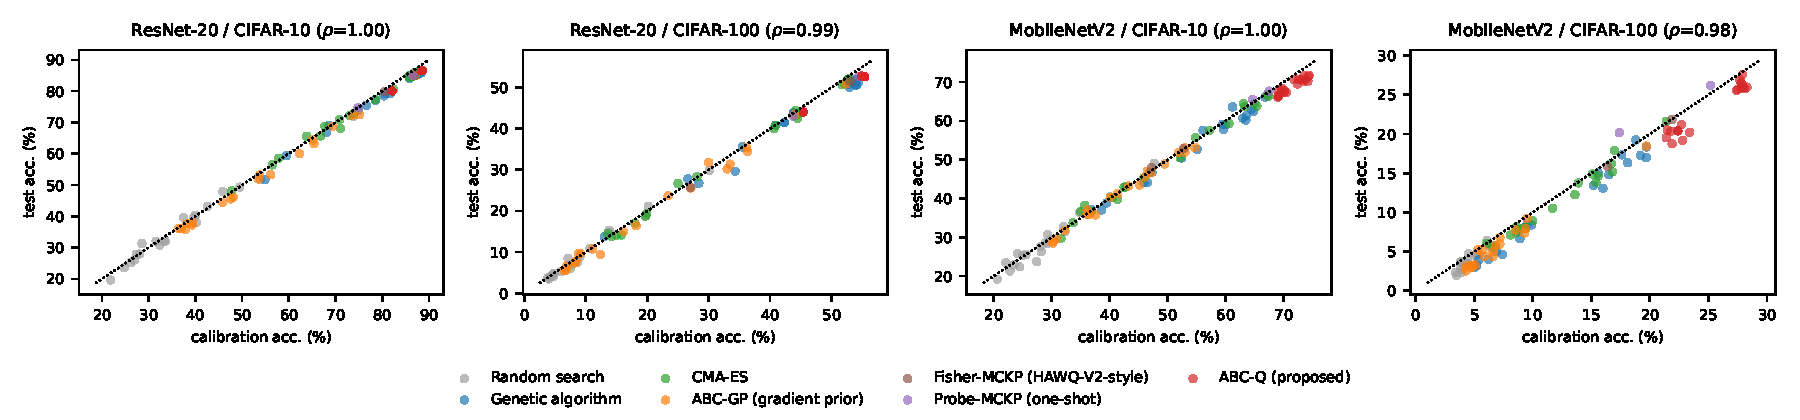
\includegraphics[width=\linewidth]{figs/calib_vs_test.pdf}
\caption{Calibration vs.\ test accuracy of every returned configuration ($\beta\in\{0.25,0.35\}$, all
methods and seeds). The dotted line is $y=x$.}
\label{fig:gap}
\end{figure}

\subsection{Search dynamics}

\begin{figure}[t]
\centering
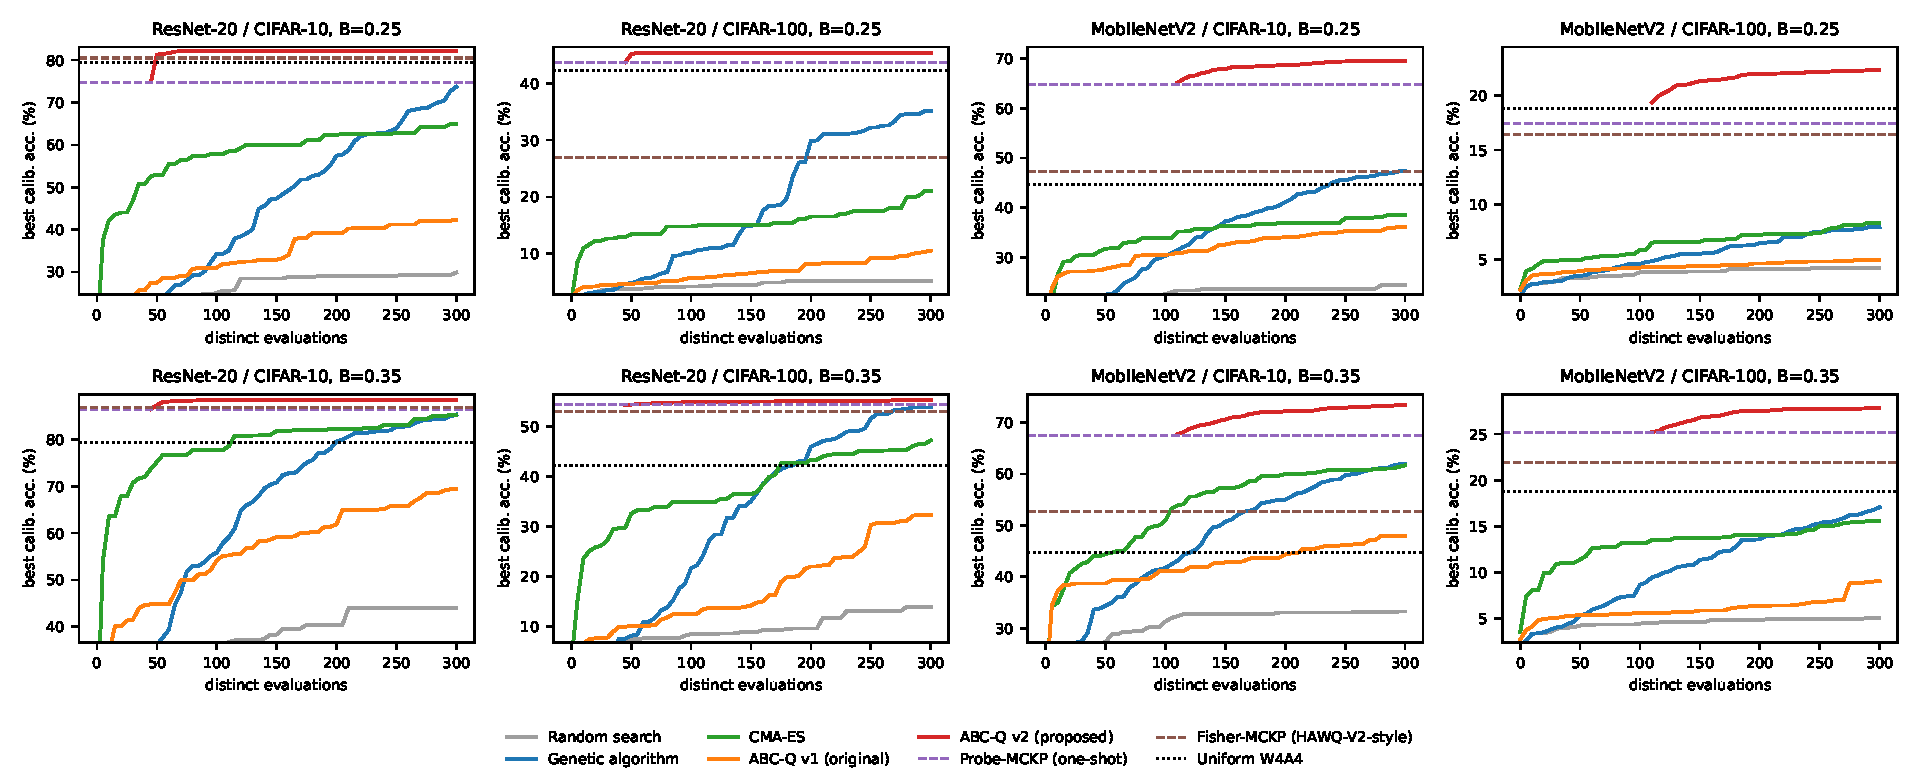
\includegraphics[width=\linewidth]{figs/anytime.pdf}
\caption{Best feasible calibration accuracy vs.\ number of distinct evaluations (mean over seeds).
ABC-Q v2 curves start after the $2L{+}1$ probe evaluations. Dashed: one-shot allocators; dotted:
uniform W4A4.}
\label{fig:anytime}
\end{figure}

Figure~\ref{fig:anytime} shows best-so-far calibration accuracy against evaluations. ABC-Q v2 spends
its first $2L+1$ evaluations on probes, yet overtakes every other method within the first few dozen
evaluations after them, because its very first food source (the MCKP optimum of the probe surrogate)
is already a strong configuration. The remaining budget yields smaller, steady gains on MobileNetV2;
on ResNet-20 the best configuration is typically found within 50--70 evaluations and never improved
upon, which indicates that the budget-constrained landscape of this homogeneous network is easy once
the probes are known.

\subsection{Component ablation}
\label{sec:ablation}

\begin{table}[t]
\centering
\caption{Component ablation of ABC-Q v2 (calibration and test accuracy, \%, mean $\pm$ std over seeds; $\Delta$: change in calibration accuracy vs.\ the full method; $p$: Holm-corrected two-sided Wilcoxon).}
\label{tab:ablation}
\footnotesize\setlength{\tabcolsep}{3pt}
\resizebox{\linewidth}{!}{\begin{tabular}{lcccc}
\toprule
Variant & Calib.\ (\%) & Test (\%) & $\Delta$ (pp) & $p$ \\
\midrule
\multicolumn{5}{l}{\emph{ResNet-20 / CIFAR-100, $B=0.25$}} \\
ABC-Q v2 (full) & 45.40 $\pm$ 0.00 & 44.03 $\pm$ 0.00 & +0.00 & -- \\
-- surrogate screening & 45.40 $\pm$ 0.00 & 44.03 $\pm$ 0.00 & +0.00 & 1.000 \\
-- online surrogate refit & 45.40 $\pm$ 0.00 & 44.03 $\pm$ 0.00 & +0.00 & 1.000 \\
-- knapsack initialisation & 45.29 $\pm$ 0.35 & 43.97 $\pm$ 0.19 & -0.11 & 1.000 \\
-- information sharing & 45.40 $\pm$ 0.00 & 44.03 $\pm$ 0.00 & +0.00 & 1.000 \\
single source (hill climber) & 45.40 $\pm$ 0.00 & 44.03 $\pm$ 0.00 & +0.00 & 1.000 \\
\midrule
\multicolumn{5}{l}{\emph{MobileNetV2 / CIFAR-10, $B=0.25$}} \\
ABC-Q v2 (full) & 69.57 $\pm$ 0.55 & 67.19 $\pm$ 0.81 & +0.00 & -- \\
-- surrogate screening & 69.36 $\pm$ 0.69 & 67.34 $\pm$ 0.61 & -0.21 & 0.516 \\
-- online surrogate refit & 68.62 $\pm$ 0.27 & 66.82 $\pm$ 0.33 & -0.95 & 0.010 \\
-- knapsack initialisation & 61.75 $\pm$ 4.61 & 61.08 $\pm$ 4.66 & -7.82 & 0.010 \\
-- information sharing & 69.89 $\pm$ 0.57 & 67.51 $\pm$ 0.22 & +0.32 & 0.176 \\
single source (hill climber) & 69.93 $\pm$ 0.85 & 67.23 $\pm$ 0.49 & +0.36 & 0.516 \\
\bottomrule
\end{tabular}}
\end{table}


Table~\ref{tab:ablation} removes one component at a time. Two components are essential:
replacing knapsack seeding (and knapsack scouts) by random feasible configurations costs $7.8$\,pp of
calibration accuracy on MobileNetV2/CIFAR-10 and increases the seed-to-seed standard deviation
eightfold ($0.55\to4.61$\,pp); freezing the surrogate at
the probe values (no online refit) costs $1.0$\,pp ($p=0.010$). Surrogate screening, the
information-sharing move and the colony itself are \emph{not} significant at this budget: a
single-source variant (a surrogate-guided hill climber started from the MCKP optimum) is statistically
indistinguishable from the full colony. On ResNet-20/CIFAR-100 all variants return essentially the same
configuration (one seed of the no-knapsack variant differs by $1.1$\,pp). We therefore attribute the performance of ABC-Q v2 to the combination of measured
probes, exact knapsack seeding and the online ridge-to-prior surrogate, and regard the ABC colony as
one adequate, but not uniquely necessary, search engine on top of them. Whether population diversity
pays off at larger evaluation budgets or on larger networks is an open question.

\subsection{How good are cheap sensitivity proxies?}

\begin{table}[t]
\centering
\caption{Do cheap sensitivity proxies predict the measured single-layer accuracy drop $\Delta_i(b)$? Spearman rank correlation $\rho$ between the gradient-magnitude prior $\tilde s_i$ (resp.\ the HAWQ-V2-style Fisher score $\Omega_i(b)$) and $\Delta_i(b)$, and overlap between the gradient-prior top-25\% `sensitive' set and the 25\% of layers with the largest measured 2-bit drop.}
\label{tab:sens_corr}
\footnotesize
\resizebox{\linewidth}{!}{\begin{tabular}{lccccccc}
\toprule
Model & $L$ & $\rho(\tilde s,\Delta_4)$ & $\rho(\tilde s,\Delta_2)$ & $\rho(\Omega_4,\Delta_4)$ & $\rho(\Omega_2,\Delta_2)$ & Top-25\% overlap \\
\midrule
ResNet-20 / CIFAR-10 & 22 & 0.57 & 0.40 & -0.08 & 0.59 & 0.50 \\
ResNet-20 / CIFAR-100 & 22 & 0.17 & 0.35 & 0.06 & 0.49 & 0.33 \\
MobileNetV2 / CIFAR-10 & 53 & 0.48 & 0.61 & 0.41 & 0.64 & 0.57 \\
MobileNetV2 / CIFAR-100 & 53 & 0.19 & 0.38 & 0.03 & 0.42 & 0.50 \\
\bottomrule
\end{tabular}}
\end{table}


Table~\ref{tab:sens_corr} tests the assumption behind ABC-Q v1 and HAWQ-style allocation. The v1
gradient-magnitude prior correlates only moderately with the measured 2-bit damage
($\rho=0.35$--$0.61$) and weakly with the 4-bit damage on ResNet-20/CIFAR-100 ($\rho=0.17$); its
top-25\% ``sensitive'' set overlaps with the truly most damaging layers in only 33--57\% of cases. The
Fisher-weighted quantization-error score is similar for 2 bits ($\rho=0.49$--$0.64$) but nearly
uncorrelated for 4 bits on ResNet-20 ($\rho\in\{-0.08,0.06\}$). This explains both the weak v1 results
and the inconsistent Fisher-MCKP results: when the ranking of layers is wrong, an exact allocation of a
wrong objective is still wrong. Measuring the damage directly costs $2L+1$ forward passes and removes
this source of error.

\begin{figure}[t]
\centering
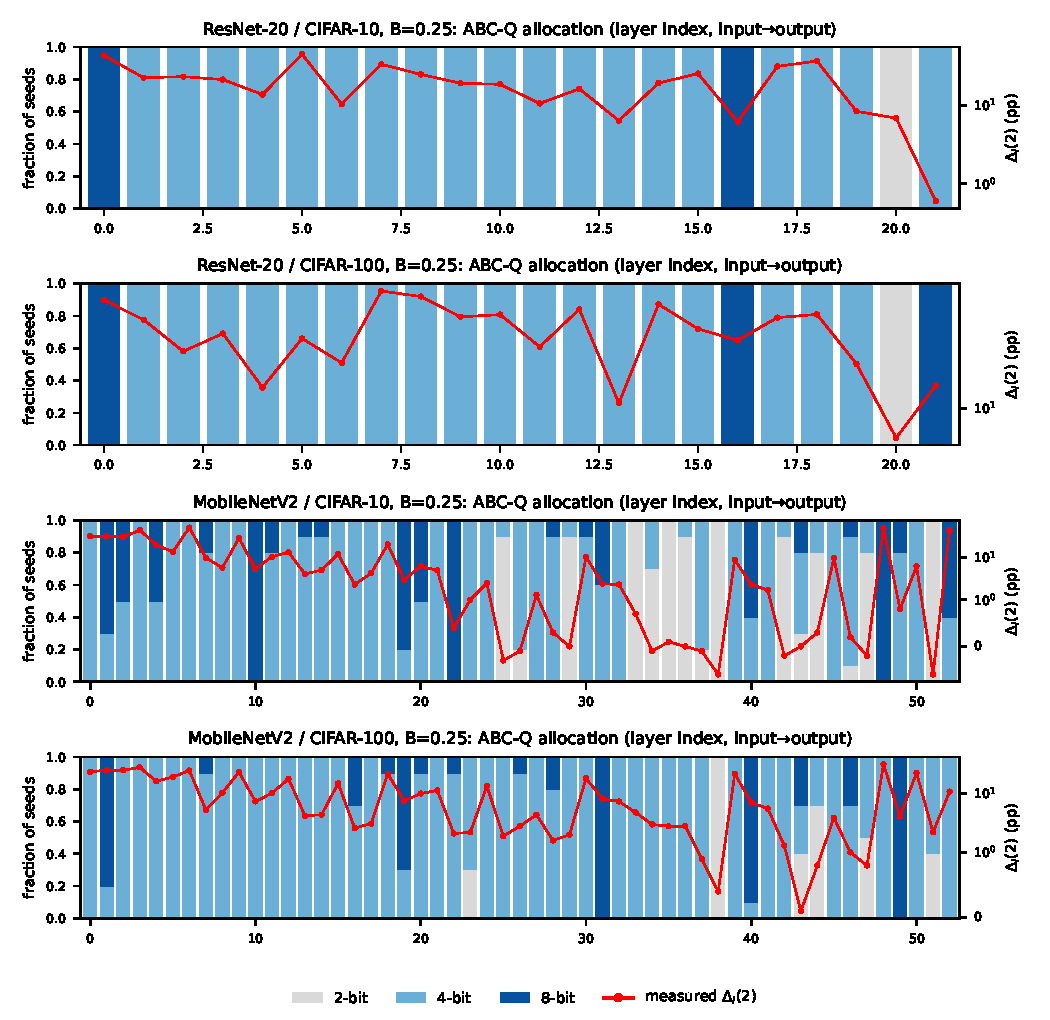
\includegraphics[width=\linewidth]{figs/bit_allocation.pdf}
\caption{Per-layer bit-widths chosen by ABC-Q v2 at $\beta=0.25$ (fraction of seeds) and the measured
single-layer 2-bit damage $\Delta_i(2)$ (red, symmetric-log scale).}
\label{fig:bits}
\end{figure}

Figure~\ref{fig:bits} shows the resulting allocations. Under the tight budget, precision is moved
into a few layers whose measured 2-bit damage is large (typically the first convolution and, in
MobileNetV2, early depthwise and projection layers), and paid for by the cheapest 2-bit layers in
compute-heavy positions.

\subsection{Quantization-aware fine-tuning}

\begin{table*}[t]
\centering
\caption{Test accuracy (\%) of the configuration found at $B=0.25$ before (PTQ) and after two epochs of quantization-aware fine-tuning (QAT, STE, network kept quantized). One configuration per method (median-calibration seed).}
\label{tab:qat}
\footnotesize\setlength{\tabcolsep}{4pt}
\resizebox{\linewidth}{!}{\begin{tabular}{lcccccccc}
\toprule
 & \multicolumn{2}{c}{ResNet-20 / CIFAR-10} & \multicolumn{2}{c}{ResNet-20 / CIFAR-100} & \multicolumn{2}{c}{MobileNetV2 / CIFAR-10} & \multicolumn{2}{c}{MobileNetV2 / CIFAR-100} \\
Configuration & PTQ & QAT & PTQ & QAT & PTQ & QAT & PTQ & QAT \\
\midrule
Uniform W4A4 & 79.73 & 86.35 & 41.47 & 55.08 & 44.09 & 71.15 & 20.44 & 29.32 \\
Fisher-MCKP & 79.83 & 87.25 & 25.71 & 54.38 & 47.91 & 70.94 & 15.85 & 29.11 \\
GA & 77.05 & 86.50 & 40.83 & 54.85 & 46.71 & 65.13 & 4.66 & 22.30 \\
CMA-ES & 68.78 & 86.44 & 18.73 & 50.31 & 40.31 & 65.43 & 8.15 & 24.44 \\
ABC-Q v2 & 80.05 & 87.41 & 44.03 & 55.87 & 67.95 & 69.72 & 20.39 & 29.48 \\
\bottomrule
\end{tabular}}
\end{table*}


Table~\ref{tab:qat} reports test accuracy after two epochs of QAT. QAT recovers most of the
post-training loss for every configuration and compresses the differences between allocators to
$\le1.5$\,pp for all methods except CMA-ES and GA on the hardest settings. After QAT, the ABC-Q v2
configuration is the best of the five on both ResNet-20 tasks ($87.41\%$ vs.\ $86.35\%$ for uniform
W4A4 on CIFAR-10; $55.87\%$ vs.\ $55.08\%$ on CIFAR-100) and tied-best on MobileNetV2/CIFAR-100
($29.48\%$ vs.\ $29.32\%$), whereas on MobileNetV2/CIFAR-10 uniform W4A4 recovers better ($71.15\%$
vs.\ $69.72\%$); mixed configurations that trade 2-bit layers for 8-bit layers are not always easier to
fine-tune than uniform 4-bit. The practical message is that ABC-Q v2 is above all a
\emph{post-training} method: without any gradient-based training it reaches, on MobileNetV2/CIFAR-10,
$95\%$ of the accuracy that uniform W4A4 attains only after QAT, while with a QAT budget its advantage
shrinks to about one percentage point in either direction. These QAT results use one configuration per
method and a short schedule and should be read as indicative; putting fine-tuning inside the search
loop is the natural next step.

\subsection{Cost}

\begin{table}[t]
\centering
\caption{Mean wall-clock time per search run (s) on an Apple M4 laptop (16\,GB). All stochastic methods use the same number of distinct evaluations, so wall time is dominated by forward passes; ABC-Q includes probes and surrogate overhead.}
\label{tab:wall}
\footnotesize\setlength{\tabcolsep}{2.5pt}
\resizebox{\linewidth}{!}{\begin{tabular}{lccccccc}
\toprule
Model & Random & GA & CMA-ES & ABC-GP & Fisher & Probe & ABC-Q \\
\midrule
ResNet-20 / CIFAR-10 & 167 & 169 & 172 & 214 & 1 & 1 & 206 \\
ResNet-20 / CIFAR-100 & 220 & 169 & 175 & 172 & 1 & 1 & 160 \\
MobileNetV2 / CIFAR-10 & 131 & 136 & 147 & 172 & 1 & 1 & 116 \\
MobileNetV2 / CIFAR-100 & 64 & 64 & 64 & 64 & 0 & 0 & 43 \\
\bottomrule
\end{tabular}}
\end{table}


Table~\ref{tab:wall} reports wall-clock times. Because all search methods are limited to the same
number of distinct evaluations, their run times are similar (2--5 minutes per run on a laptop); the
surrogate, knapsack and refit computations of ABC-Q v2 add no measurable overhead (its runs are not
slower than those of the baselines). The one-shot allocators need seconds after their statistics are computed.

\subsection{Limitations}
\begin{itemize}
\item \textbf{Scale.} All experiments use $32\times32$ CIFAR images and two compact backbones trained
      for 40 epochs; our MobileNetV2/CIFAR-100 float model is weak ($35.9\%$). ImageNet-scale
      validation with stronger checkpoints is required before deployment claims.
\item \textbf{Simulated quantization and BOPs.} We use fake quantization without BatchNorm folding and
      MAC-weighted BOPs as the cost; measured latency or energy on a specific accelerator may rank
      configurations differently.
\item \textbf{The colony is not the source of the gain.} As shown by the ablation, a single-source
      surrogate-guided search performs as well as the colony at $E=300$.
\item \textbf{Seeds.} All search comparisons use ten seeds, but QAT uses one configuration per method
      and two epochs.
\item \textbf{PTQ scope.} After QAT the differences between allocations shrink to about one
      percentage point, and uniform 4-bit is better on MobileNetV2/CIFAR-10.
\end{itemize}

%% ===================================================================================
\section{Conclusion}
%% ===================================================================================
We revisited swarm-based mixed-precision bit allocation under a hard BOPs budget and an equal
evaluation budget for every method. Unguided metaheuristics (random search, a GA, CMA-ES and our
earlier ABC-Q v1) turned out to be worse than simply quantizing every layer to 4 bits at the same
cost. ABC-Q v2, which measures single-layer damage directly, seeds its population with exact
multiple-choice-knapsack optima of an additive surrogate and refits that surrogate online, was the
best or tied-best method in all settings, with large gains on the heterogeneous MobileNetV2
($+23$\,pp test accuracy over uniform W4A4 at equal cost on CIFAR-10) and small gains on the homogeneous
ResNet-20. The ablation shows that probes, knapsack seeding and the online surrogate, rather than the
colony dynamics, carry the improvement, and the QAT experiment shows that the advantage is largest in
the post-training setting and shrinks to about one percentage point after fine-tuning. We also found that the gradient-magnitude prior used by v1 and a
Fisher-weighted HAWQ-style score are only moderately correlated with measured damage.

Future work should (i) validate on ImageNet-scale models with hardware-measured latency,
(ii) put short fine-tuning inside the search loop, (iii) study larger evaluation budgets where
population diversity may matter, and (iv) combine the searched allocation with reconstruction-based
PTQ such as AdaRound or BRECQ \citep{Nagel2020AdaRound,Li2021BRECQ}.

\appendix
\section{Per-configuration results}
\label{app:tables}
\FloatBarrier
\begin{table}[t]
\centering
\caption{ResNet-20 / CIFAR-10, BOPs budget $B=0.25$ (fraction of W8A8), $E=300$ evaluations, $n=10$ seeds. Float test accuracy 88.98\%. Calib./test: PTQ accuracy (no fine-tuning) on the 1k calibration and 10k test sets. $p$: Holm-corrected two-sided Wilcoxon vs.\ ABC-Q v2 on calibration accuracy; $A_{12}$: Vargha--Delaney effect size (probability that v2 is better). Friedman $p=9.6e-08$.}
\label{tab:main_resnet20_cifar10_B250}
\footnotesize\setlength{\tabcolsep}{3.5pt}
\resizebox{\linewidth}{!}{\begin{tabular}{lcccccc}
\toprule
Method & Calib.\ acc.\ (\%) & Test acc.\ (\%) & BOPs & Bits/param & $p$ & $A_{12}$ \\
\midrule
Uniform W4A4 & 79.40 & 79.73 & 0.250 & 4.00 & -- & -- \\
Random search & 29.84 $\pm$ 7.61 & 29.49 $\pm$ 8.00 & 0.234 & 3.64 & 0.008 & 1.00 \\
Genetic algorithm & 73.72 $\pm$ 9.70 & 72.11 $\pm$ 9.72 & 0.249 & 3.88 & 0.008 & 0.95 \\
CMA-ES & 64.93 $\pm$ 8.48 & 64.74 $\pm$ 7.99 & 0.241 & 3.90 & 0.008 & 1.00 \\
ABC-Q v1 (original) & 42.31 $\pm$ 5.93 & 40.86 $\pm$ 5.66 & 0.235 & 3.79 & 0.008 & 1.00 \\
Fisher-MCKP (HAWQ-V2-style) & 80.50 & 79.83 & 0.247 & 3.74 & -- & -- \\
Probe-MCKP (one-shot) & 74.80 & 74.70 & 0.247 & 3.94 & -- & -- \\
\textbf{ABC-Q v2 (proposed)} & \textbf{82.10 $\pm$ 0.00} & \textbf{80.05 $\pm$ 0.00} & 0.250 & 3.76 & -- & -- \\
\bottomrule
\end{tabular}}
\end{table}

\begin{table}[t]
\centering
\caption{ResNet-20 / CIFAR-10, BOPs budget $B=0.35$ (fraction of W8A8), $E=300$ evaluations, $n=10$ seeds. Float test accuracy 88.98\%. Calib./test: PTQ accuracy (no fine-tuning) on the 1k calibration and 10k test sets. $p$: Holm-corrected two-sided Wilcoxon vs.\ ABC-Q v2 on calibration accuracy; $A_{12}$: Vargha--Delaney effect size (probability that v2 is better). Friedman $p=3.4e-07$.}
\label{tab:main_resnet20_cifar10_B350}
\footnotesize\setlength{\tabcolsep}{3.5pt}
\resizebox{\linewidth}{!}{\begin{tabular}{lcccccc}
\toprule
Method & Calib.\ acc.\ (\%) & Test acc.\ (\%) & BOPs & Bits/param & $p$ & $A_{12}$ \\
\midrule
Uniform W4A4 & 79.40 & 79.73 & 0.250 & 4.00 & -- & -- \\
Random search & 43.96 $\pm$ 12.14 & 43.52 $\pm$ 11.83 & 0.336 & 4.57 & 0.008 & 1.00 \\
Genetic algorithm & 85.31 $\pm$ 5.93 & 83.66 $\pm$ 5.18 & 0.330 & 4.34 & 0.008 & 0.97 \\
CMA-ES & 85.31 $\pm$ 2.80 & 83.86 $\pm$ 2.77 & 0.336 & 4.56 & 0.008 & 1.00 \\
ABC-Q v1 (original) & 69.44 $\pm$ 11.36 & 67.77 $\pm$ 11.34 & 0.321 & 4.29 & 0.008 & 1.00 \\
Fisher-MCKP (HAWQ-V2-style) & 86.90 & 85.07 & 0.347 & 5.13 & -- & -- \\
Probe-MCKP (one-shot) & 86.50 & 85.01 & 0.347 & 4.08 & -- & -- \\
\textbf{ABC-Q v2 (proposed)} & \textbf{88.50 $\pm$ 0.11} & \textbf{86.60 $\pm$ 0.04} & 0.348 & 4.27 & -- & -- \\
\bottomrule
\end{tabular}}
\end{table}

\begin{table}[t]
\centering
\caption{ResNet-20 / CIFAR-100, BOPs budget $B=0.25$ (fraction of W8A8), $E=300$ evaluations, $n=10$ seeds. Float test accuracy 59.73\%. Calib./test: PTQ accuracy (no fine-tuning) on the 1k calibration and 10k test sets. $p$: Holm-corrected two-sided Wilcoxon vs.\ ABC-Q on calibration accuracy; $A_{12}$: Vargha--Delaney effect size (probability that ABC-Q is better). Friedman $p=2.6e-07$.}
\label{tab:main_resnet20_cifar100_B250}
\footnotesize\setlength{\tabcolsep}{3.5pt}
\resizebox{\linewidth}{!}{\begin{tabular}{lcccccc}
\toprule
Method & Calib.\ acc.\ (\%) & Test acc.\ (\%) & BOPs & Bits/param & $p$ & $A_{12}$ \\
\midrule
Uniform W4A4 & 42.30 & 41.47 & 0.250 & 4.00 & -- & -- \\
Random search & 5.28 $\pm$ 1.49 & 5.11 $\pm$ 1.71 & 0.237 & 3.69 & 0.008 & 1.00 \\
Genetic algorithm & 35.09 $\pm$ 9.97 & 34.48 $\pm$ 9.84 & 0.247 & 3.95 & 0.008 & 1.00 \\
CMA-ES & 21.02 $\pm$ 8.42 & 20.74 $\pm$ 8.77 & 0.237 & 3.89 & 0.008 & 1.00 \\
ABC-GP (gradient prior) & 10.53 $\pm$ 6.12 & 9.77 $\pm$ 5.83 & 0.230 & 3.85 & 0.008 & 1.00 \\
Fisher-MCKP (HAWQ-V2-style) & 27.00 & 25.71 & 0.244 & 4.11 & -- & -- \\
Probe-MCKP (one-shot) & 43.70 & 43.06 & 0.247 & 3.83 & -- & -- \\
\textbf{ABC-Q (proposed)} & \textbf{45.40 $\pm$ 0.00} & \textbf{44.03 $\pm$ 0.00} & 0.250 & 3.86 & -- & -- \\
\bottomrule
\end{tabular}}
\end{table}

\begin{table}[t]
\centering
\caption{ResNet-20 / CIFAR-100, BOPs budget $B=0.35$ (fraction of W8A8), $E=300$ evaluations, $n=10$ seeds. Float test accuracy 59.73\%. Calib./test: PTQ accuracy (no fine-tuning) on the 1k calibration and 10k test sets. $p$: Holm-corrected two-sided Wilcoxon vs.\ ABC-Q on calibration accuracy; $A_{12}$: Vargha--Delaney effect size (probability that ABC-Q is better). Friedman $p=9.8e-08$.}
\label{tab:main_resnet20_cifar100_B350}
\footnotesize\setlength{\tabcolsep}{3.5pt}
\resizebox{\linewidth}{!}{\begin{tabular}{lcccccc}
\toprule
Method & Calib.\ acc.\ (\%) & Test acc.\ (\%) & BOPs & Bits/param & $p$ & $A_{12}$ \\
\midrule
Uniform W4A4 & 42.30 & 41.47 & 0.250 & 4.00 & -- & -- \\
Random search & 13.98 $\pm$ 7.46 & 13.86 $\pm$ 7.77 & 0.332 & 4.37 & 0.008 & 1.00 \\
Genetic algorithm & 53.82 $\pm$ 0.73 & 51.16 $\pm$ 0.76 & 0.335 & 4.35 & 0.008 & 0.94 \\
CMA-ES & 47.22 $\pm$ 4.55 & 46.34 $\pm$ 4.55 & 0.331 & 4.44 & 0.008 & 1.00 \\
ABC-GP (gradient prior) & 32.30 $\pm$ 11.13 & 31.24 $\pm$ 11.07 & 0.327 & 4.41 & 0.008 & 1.00 \\
Fisher-MCKP (HAWQ-V2-style) & 53.00 & 51.47 & 0.347 & 5.19 & -- & -- \\
Probe-MCKP (one-shot) & 54.40 & \textbf{52.73} & 0.328 & 4.24 & -- & -- \\
\textbf{ABC-Q (proposed)} & \textbf{55.30 $\pm$ 0.21} & 52.64 $\pm$ 0.07 & 0.350 & 4.26 & -- & -- \\
\bottomrule
\end{tabular}}
\end{table}

\begin{table}[t]
\centering
\caption{MobileNetV2 / CIFAR-10, BOPs budget $B=0.25$ (fraction of W8A8), $E=300$ evaluations, $n=10$ seeds. Float test accuracy 76.32\%. Calib./test: PTQ accuracy (no fine-tuning) on the 1k calibration and 10k test sets. $p$: Holm-corrected two-sided Wilcoxon vs.\ ABC-Q v2 on calibration accuracy; $A_{12}$: Vargha--Delaney effect size (probability that v2 is better). Friedman $p=3e-07$.}
\label{tab:main_mobilenetv2_cifar10_B250}
\footnotesize\setlength{\tabcolsep}{3.5pt}
\resizebox{\linewidth}{!}{\begin{tabular}{lcccccc}
\toprule
Method & Calib.\ acc.\ (\%) & Test acc.\ (\%) & BOPs & Bits/param & $p$ & $A_{12}$ \\
\midrule
Uniform W4A4 & 44.70 & 44.09 & 0.250 & 4.00 & -- & -- \\
Random search & 24.37 $\pm$ 2.30 & 23.73 $\pm$ 2.47 & 0.244 & 3.32 & 0.008 & 1.00 \\
Genetic algorithm & 47.31 $\pm$ 7.98 & 46.21 $\pm$ 7.82 & 0.240 & 3.34 & 0.008 & 1.00 \\
CMA-ES & 38.58 $\pm$ 4.65 & 38.63 $\pm$ 4.68 & 0.244 & 3.40 & 0.008 & 1.00 \\
ABC-Q v1 (original) & 36.21 $\pm$ 5.52 & 35.55 $\pm$ 5.78 & 0.239 & 3.23 & 0.008 & 1.00 \\
Fisher-MCKP (HAWQ-V2-style) & 47.20 & 47.91 & 0.247 & 3.60 & -- & -- \\
Probe-MCKP (one-shot) & 64.70 & 65.47 & 0.247 & 3.32 & -- & -- \\
\textbf{ABC-Q v2 (proposed)} & \textbf{69.57 $\pm$ 0.55} & \textbf{67.19 $\pm$ 0.81} & 0.249 & 3.39 & -- & -- \\
\bottomrule
\end{tabular}}
\end{table}

\begin{table}[t]
\centering
\caption{MobileNetV2 / CIFAR-10, BOPs budget $B=0.35$ (fraction of W8A8), $E=300$ evaluations, $n=10$ seeds. Float test accuracy 76.32\%. Calib./test: PTQ accuracy (no fine-tuning) on the 1k calibration and 10k test sets. $p$: Holm-corrected two-sided Wilcoxon vs.\ ABC-Q on calibration accuracy; $A_{12}$: Vargha--Delaney effect size (probability that ABC-Q is better). Friedman $p=2.1e-07$.}
\label{tab:main_mobilenetv2_cifar10_B350}
\footnotesize\setlength{\tabcolsep}{3.5pt}
\resizebox{\linewidth}{!}{\begin{tabular}{lcccccc}
\toprule
Method & Calib.\ acc.\ (\%) & Test acc.\ (\%) & BOPs & Bits/param & $p$ & $A_{12}$ \\
\midrule
Uniform W4A4 & 44.70 & 44.09 & 0.250 & 4.00 & -- & -- \\
Random search & 33.26 $\pm$ 6.21 & 33.36 $\pm$ 6.90 & 0.342 & 3.93 & 0.008 & 1.00 \\
Genetic algorithm & 61.86 $\pm$ 3.80 & 60.67 $\pm$ 3.71 & 0.336 & 3.76 & 0.008 & 1.00 \\
CMA-ES & 61.63 $\pm$ 5.29 & 61.25 $\pm$ 5.31 & 0.344 & 3.96 & 0.008 & 1.00 \\
ABC-GP (gradient prior) & 47.96 $\pm$ 5.67 & 47.41 $\pm$ 5.76 & 0.337 & 3.77 & 0.008 & 1.00 \\
Fisher-MCKP (HAWQ-V2-style) & 52.70 & 52.79 & 0.348 & 3.99 & -- & -- \\
Probe-MCKP (one-shot) & 67.50 & 67.68 & 0.346 & 3.52 & -- & -- \\
\textbf{ABC-Q (proposed)} & \textbf{73.37 $\pm$ 0.87} & \textbf{70.71 $\pm$ 0.69} & 0.348 & 3.76 & -- & -- \\
\bottomrule
\end{tabular}}
\end{table}

\begin{table}[t]
\centering
\caption{MobileNetV2 / CIFAR-100, BOPs budget $B=0.25$ (fraction of W8A8), $E=300$ evaluations, $n=10$ seeds. Float test accuracy 48.90\%. Calib./test: PTQ accuracy (no fine-tuning) on the 1k calibration and 10k test sets. $p$: Holm-corrected two-sided Wilcoxon vs.\ ABC-Q on calibration accuracy; $A_{12}$: Vargha--Delaney effect size (probability that ABC-Q is better). Friedman $p=1.9e-06$.}
\label{tab:main_mobilenetv2_cifar100_B250}
\footnotesize\setlength{\tabcolsep}{3.5pt}
\resizebox{\linewidth}{!}{\begin{tabular}{lcccccc}
\toprule
Method & Calib.\ acc.\ (\%) & Test acc.\ (\%) & BOPs & Bits/param & $p$ & $A_{12}$ \\
\midrule
Uniform W4A4 & 19.90 & 19.63 & 0.250 & 4.00 & -- & -- \\
Random search & 3.01 $\pm$ 0.40 & 1.93 $\pm$ 0.49 & 0.242 & 3.44 & 0.008 & 1.00 \\
Genetic algorithm & 5.50 $\pm$ 2.54 & 3.73 $\pm$ 2.52 & 0.240 & 3.37 & 0.008 & 1.00 \\
CMA-ES & 5.04 $\pm$ 1.09 & 4.24 $\pm$ 1.61 & 0.243 & 3.59 & 0.008 & 1.00 \\
ABC-GP (gradient prior) & 3.48 $\pm$ 0.39 & 2.22 $\pm$ 0.34 & 0.238 & 3.39 & 0.008 & 1.00 \\
Fisher-MCKP (HAWQ-V2-style) & 19.20 & 20.13 & 0.248 & 3.97 & -- & -- \\
Probe-MCKP (one-shot) & 27.00 & 24.35 & 0.248 & 3.68 & -- & -- \\
\textbf{ABC-Q (proposed)} & \textbf{27.27 $\pm$ 0.35} & \textbf{24.65 $\pm$ 0.37} & 0.249 & 3.70 & -- & -- \\
\bottomrule
\end{tabular}}
\end{table}

\begin{table}[t]
\centering
\caption{MobileNetV2 / CIFAR-100, BOPs budget $B=0.35$ (fraction of W8A8), $E=300$ evaluations, $n=10$ seeds. Float test accuracy 48.90\%. Calib./test: PTQ accuracy (no fine-tuning) on the 1k calibration and 10k test sets. $p$: Holm-corrected two-sided Wilcoxon vs.\ ABC-Q on calibration accuracy; $A_{12}$: Vargha--Delaney effect size (probability that ABC-Q is better). Friedman $p=2e-07$.}
\label{tab:main_mobilenetv2_cifar100_B350}
\footnotesize\setlength{\tabcolsep}{3.5pt}
\resizebox{\linewidth}{!}{\begin{tabular}{lcccccc}
\toprule
Method & Calib.\ acc.\ (\%) & Test acc.\ (\%) & BOPs & Bits/param & $p$ & $A_{12}$ \\
\midrule
Uniform W4A4 & 19.90 & 19.63 & 0.250 & 4.00 & -- & -- \\
Random search & 4.49 $\pm$ 1.34 & 3.56 $\pm$ 1.17 & 0.341 & 4.09 & 0.008 & 1.00 \\
Genetic algorithm & 13.99 $\pm$ 4.08 & 12.39 $\pm$ 4.08 & 0.336 & 4.13 & 0.008 & 1.00 \\
CMA-ES & 13.58 $\pm$ 1.50 & 13.59 $\pm$ 1.70 & 0.334 & 4.20 & 0.008 & 1.00 \\
ABC-GP (gradient prior) & 6.54 $\pm$ 2.59 & 5.34 $\pm$ 2.98 & 0.341 & 3.92 & 0.008 & 1.00 \\
Fisher-MCKP (HAWQ-V2-style) & 28.20 & 30.04 & 0.347 & 5.04 & -- & -- \\
Probe-MCKP (one-shot) & 31.10 & 32.03 & 0.346 & 4.30 & -- & -- \\
\textbf{ABC-Q (proposed)} & \textbf{34.23 $\pm$ 0.64} & \textbf{32.61 $\pm$ 0.55} & 0.349 & 4.23 & -- & -- \\
\bottomrule
\end{tabular}}
\end{table}

\FloatBarrier

\section*{Declarations}
\paragraph{Funding} No funding was received for this work.
\paragraph{Competing interests} The authors declare no competing interests.
\paragraph{Data and code availability} CIFAR-10/100 are public. Code, raw per-run results and
configurations will be made available in a public repository upon publication.
\paragraph{Author contributions} \emph{(fill in using CRediT roles before submission)}

\section*{Acknowledgements}
The authors thank Professor Richa Bhatiya for teaching the optimization course that grounded the
algorithmic ideas in this work.

\bibliographystyle{unsrtnat}
\bibliography{refs}
\end{document}
